\appendix
\chapter{Appendix}
\renewcommand\thesection{\Roman{section}}
\label{chap:appendix}
\section{Derivation of the threshold $t$ for non-amplified LSH schemes}
\label{appendix:derivation_threshold}
In Section \ref{section:lit:introducing_lsh} we aim to solve Equation \ref{eq:identifying_equation}. To do this, we first derive $\frac{\partial 1 - (1-s^r)^b}{\partial s}$

\begin{align*}
    \frac{\partial 1 - (1-s^r)^b}{\partial s} &= -\frac{\partial (1-s^r)^b}{\partial (1-s^r)} \frac{(1-s^r)}{\partial (s)}\\
                                &= - b(1-s^r)^{b -1 } * - rs^{r-1}\\
                                &= b(1-s^r)^{b -1 } rs^{r-1}
\end{align*}


This allows us to derive an expression for the second derivative $\frac{\partial^2 1 - (1-s^r)^b }{\partial s^2}$

\begin{align*}
    \frac{\partial^2 1 - (1-s^r)^b }{\partial s^2} &= \frac{\partial b(1-s^r)^{b -1 } rs^{r-1}}{\partial s} \\ 
                                    &= \frac{\partial b(1-s^r)^{b -1 } }{\partial s} rs^{r-1}  + b(1-s^r)^{b -1 } \frac{\partial rs^{r-1}}{\partial s} \\
                                    &= (b-1) b(1-s^r)^{b - 2 }rs^{r-1}  *  - rs^{r-1} + b(1-s^r)^{b -1 }  r(r-1)s^{r-2}\\
                                    &= - (b-1) b(1-s^r)^{b - 2 }r^2s^{2r-2} + b(1-s^r)^{b -1 }  r(r-1)s^{r-2}\\
\end{align*}

Substituting the formula for the second derivative into equation \ref{eq:identifying_equation}, we can now find the formula for $t$. 

\begin{align*}
    \frac{\partial^2 1 - (1-s^r)^b }{\partial s^2} = 0 &\Leftrightarrow (b-1) b(1-s^r)^{b - 2 }r^2s^{2r-2} = b(1-s^r)^{b -1 } r(r-1)s^{r-2} \\
                                        &\Leftrightarrow (b-1)rs^{r} = (r-1)(1 - s^r) \\
                                        %&\Leftrightarrow (b-1)rs^{r} = (r-1) - (r-1)s^r\\
                                        &\Leftrightarrow (b-1)rs^{r}s + (r-1)s^r = r - 1 \\
                                       % &\Leftrightarrow s^{r}(r(b-1) + r - 1) = r - 1 \\
                                        &\Leftrightarrow s^{r}(rb-1) = r -1 \\
                                        %&\Leftrightarrow s^{r} = \frac{r-1}{rb-1} \\
                                        &\Leftrightarrow \hat{s} = t = (\frac{r-1}{rb-1})^{\frac{1}{r}}
\end{align*}
\section{Derivation for second derivative of amplified s-curve}
\label{appendix:derivation_second_derivative_s_curve}
In section \ref{section:meth:amplification}, we aim to solve Equation \ref{eq:identifying_equation_amplified}.

\begin{equation}
    \frac{\partial^2 1 - (1- (1 - (1-s^{r_1})^{b_1})^{r_2})^{b_2} }{\partial s^2} = 0
\end{equation}

We first derive an expression for  $\frac{\partial 1 - (1- (1 - (1-s^{r_1})^{b_1})^{r_2})^{b_2}}{\partial s}$ by an iterative application of the chain rule
\begin{align}
    &\frac{d 1 - (1- (1 - (1-s^{r_1})^{b_1})^{r_2})^{b_2}}{ds} = -b2 *(1-(1-(1-s^{r_1})^{b_1})^{r_2})^{b_2 - 1} * \frac{(1-(1-s^{r_1})^{b_1})^{r_2}}{ds}\\
    &= -b_2 *(1-(1-(1-s^{r_1})^{b_1})^{r_2})^{b_2 - 1} * - r_2 * (1-(1-s^{r_1})^{b_1})^{r_2 - 1} *  \frac{1-(1-s^{r_1})^{b_1}}{ds} \nonumber  \\
    &= -b_2 *(1-(1-(1-s^{r_1})^{b_1})^{r_2})^{b_2 - 1} * - r_2 * (1-(1-s^{r_1})^{b_1})^{r_2 - 1} * b_1r_1(1-s^{r_1})^{b_1-1}s^{r_1-1} \nonumber\\                                                     
    &= b_1r_1b_2r_2s^{r_1-1}(1-s^{r_1})^{b_1-1}(1-(1-s^{r_1})^{b_1})^{r_2-1}(1-(1-(1-s^{r_2})^{b_1})^{r_2})^{b_2-1} \nonumber
\label{appendix:derivation_first_deriv_ampl_s_curve}
\end{align}

The second derivative of the amplified s-curve to $s$ is then given as follows
\begin{equation}
    \begin{aligned}
        &\frac{\partial^{2}}{\partial s^{2}}\left(1-\left(1-\left(1-\left(1-s^{r_1}\right)^{b_1}\right)^{r_2}\right)^{b_2}\right)= \\
        &-{r_1}^{2} {b_1}^{2} {r_2}^{2}({b_2}-1) {b_2} s^{2 {r_1}-2}\gamma^{2 {b_1}-2}\beta^{2 {r_2}-2}\alpha^{{b_2}-2}+\\
        &{r_1}^{2} {b_1}^{2}({r_2}-1) {r_2} {b_2} s^{2 {r_1}-2}\gamma^{2 {b_1}-2}\beta^{{r_2}-2}\alpha^{{b_2}-1}-\\
        &{r_1}^{2}({b_1}-1) {b_1} {r_2} {b_2} s^{2 {r_1}-2}\gamma^{{b_1}-2}\beta^{{r_2}-1}\alpha^{{b_2}-1}+\\
        &({r_1}-1) {r_1} {b_1} {r_2} {b_2} s^{{r_1}-2}\gamma^{{b_1}-1}\beta^{{r_2}-1}\alpha^{{b_2}-1} \\
        &\text{with } \alpha = (1 - (1- (1 - s^{r_1})^{b_1})^{r_2} \\
        &\text{     } \beta = 1- (1 - s^{r_1})^{b_1}\\
        &\text{     } \gamma = 1 - s^{r_1}
    \end{aligned}
\end{equation}

Setting the second derivative of the amplified s-curve equal to $0$ gives
\begin{equation}
    \begin{aligned}
        &{r_1}^{2} {b_1}^{2}({r_2}-1) {r_2} {b_2} s^{2 {r_1}-2}\gamma^{2 {b_1}-2}\beta^{{r_2}-2}\alpha^{{b_2}-1} + ({r_1}-1) {r_1} {b_1} {r_2} {b_2} s^{{r_1}-2}\gamma^{{b_1}-1}\beta^{{r_2}-1}\alpha^{{b_2}-1}  = \\
        &{r_1}^{2} {b_1}^{2} {r_2}^{2}({b_2}-1) {b_2} s^{2 {r_1}-2}\gamma^{2 {b_1}-2}\beta^{2 {r_2}-2}\alpha^{{b_2}-2} + {r_1}^{2}({b_1}-1) {b_1} {r_2} {b_2} s^{2 {r_1}-2}\gamma^{{b_1}-2}\beta^{{r_2}-1}\alpha^{{b_2}-1} \\ 
        &\Leftrightarrow\\
        & {r_1}^{2} {b_1}^{2}({r_2}-1) {r_2} {b_2} s^{r_1}\gamma^{{b_1}-1}\beta + ({r_1}-1) {r_1} {b_1} {r_2} {b_2} s^{{r_1}-2}\gamma^{{b_1}-1}\beta^{{r_2}-1}\alpha^{{b_2}-1} = \\
        & {r_1}^{2} {b_1}^{2} {r_2}^{2}({b_2}-1) {b_2} s^{r_1}\gamma^{{b_1}-1}\beta^{{r_2}-1}\alpha + {r_1}^{2}({b_1}-1) {b_1} {r_2} {b_2} s^{r_1}\gamma 
    \end{aligned}
\end{equation}

\newpage
\section{Plots of effect of amplification}
\label{appendix:plots_effect_amplification}
To save room in the thesis, we have not shown all PC-RR plots of the FSS scheme in the main thesis, but we do include them below for the interested reader.

\begin{figure}[!h]
    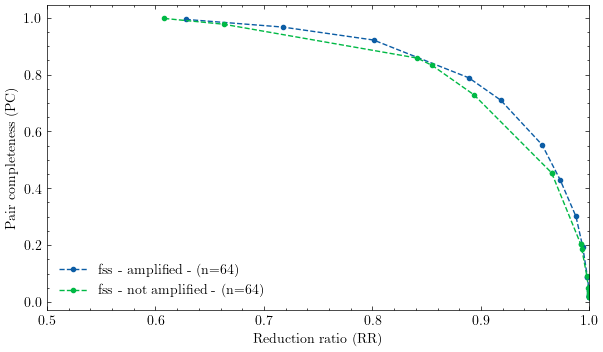
\includegraphics[width=0.75\textwidth]{fss_amplified_vs_non_amplified_64.png}
    \caption{Effect of amplification on PC and RR for the FSS scheme with $n=64$}
    \label{fig:Effect of amplification - minhash - 64}
\end{figure}

\begin{figure}[!h]
    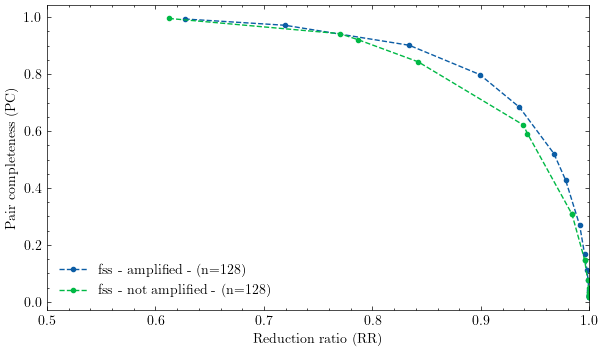
\includegraphics[width=0.75\textwidth]{fss_amplified_vs_non_amplified_128.png}
    \caption{Effect of amplification on PC and RR for the FSS scheme with $n=128$}
    \label{fig:Effect of amplification - minhash - 128}
\end{figure}

\begin{figure}[!h]
    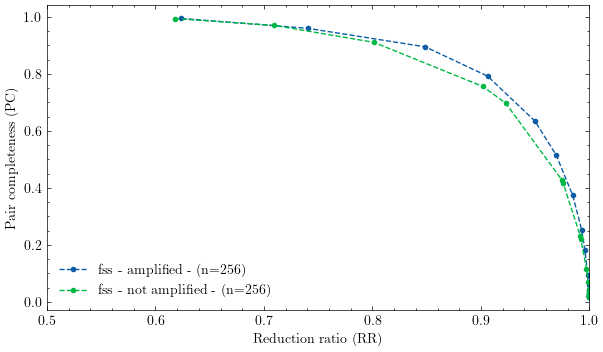
\includegraphics[width=0.75\textwidth]{fss_amplified_vs_non_amplified_256.png}
    \caption{Effect of amplification on PC and RR for the FSS scheme with $n=256$}
    \label{fig:Effect of amplification - minhash - 256}
\end{figure}

\begin{figure}[!h]
    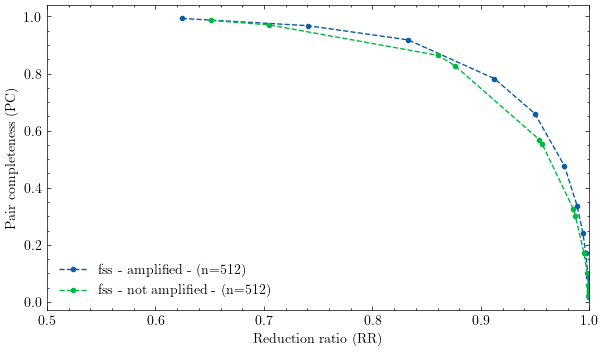
\includegraphics[width=0.75\textwidth]{fss_amplified_vs_non_amplified_512.png}
    \caption{Effect of amplification on PC and RR for the FSS scheme with $n=512$}
    \label{fig:Effect of amplification - minhash - 512}
\end{figure}
